\chapter{Explotación}

En este capítulo se expone la explotación del simulador de escenarios como método para la evaluación de sistemas de recomendaciones, el trabajo realizado para permitirlo y el rendimiento obtenido del simulador. Para más información consulte el manual del usuarios disponible en los anexos.

\section{Motivación}

Debido a la gran cantidad de información resulta difícil para los usuarios elegir entre todas las alternativas existentes en los resultados mostrados por un sistema. Por ello, para facilitar la elección se utilizan los llamados sistemas de recomendación. Estos sistemas resultan de gran interés para las empresas desde punto de vista económico, ya que hacen llegar a sus cliente recomendaciones de productos relevantes para ellos. Ademas, también resultan de interés para los usuarios ya que actúan como filtro y les ofrecen información personalizada que les resulta de interés.

No obstante, el diseño de sistemas de recomendación se enfrenta a problema como el arranque en frió (cold
start problem) o el problema de opiniones artificiales o manipuladas (spam). Esto conlleva que el sistema de recomendación muestra información no relevante para el usuario y este dejará de confiar en él y abandonarlo. 

Por esto surge la necesidad de que los sistemas de recomendaciones puedan evaluarse y calibrarse correctamente. Para que esto pueda llevarse a cabo necesitamos recolectar datos reales de escenarios reales para su posterior análisis. Este análisis consiste en calcular el error cometido por el sistema de recomendación. Una forma de cuantificar el error es con la MAE (Medium Absolute Error) que consiste en restar el valor asignado por el usuario del valor estimado por el sistema de recomendación. 

\section{Definir un escenario realista}

En este apartado se expone como definir un escenario realista con datos de restaurantes reales de la ciudad San Luis Potosí de México.

\subsection{Paso 1: obtener datos de restaurantes reales}

Lo primero que vamos a hacer es conseguir datos reales de restaurantes reales. Por esto accedemos al repositorio de Center for Machine Learning and Intelligent Systems y descargamos el siguiente archivo comprimido: \href{https://archive.ics.uci.edu/ml/machine-learning-databases/00232/RCdata.zip}{https://archive.ics.uci.edu/ml/machine-learning-databases/00232/RCdata.zip}

Una vez que hayamos descargado y descomprimido el fichero vemos que este contiene varios ficheros csv. A nosotros nos interesan los ficheros geoplaces2.csv y rating\_final.csv. El primero contiene los datos de los restaurantes y es el que vamos a importar al crea un escenario y el segundo contiene datos con valoraciones de diferentes usuarios y el que vamos a usar como datos de entrenamiento para el recomendador de ejemplo desarrollado.

\subsection{Paso 2: crear un mapa nuevo o editar un mapa existente}

Antes de todos tenemos que crear un mapa nuevo o editar uno existente para poder asociarle el escenario que vamos a crear a continuación. Por esto tenemos que usar alguna de las dos opciones:
\begin{itemize}
	\item crear un mapa nuevo: opción  Maps $\rightarrow$ new map. Para más información por favor consulte el anexo \ref{sec:crearMapa}.
	\item editar un mapa existente: opción Maps $\rightarrow$ maps search y en la lista de resultados pulsamos sobre el icono de editar imagen. Para más información por favor consulte el anexo \ref{sec:editarMapasEscenas}.
\end{itemize} 

En este caso se ha optado por crear un nuevo mapa con el nombre México ya que los datos que hemos descargado son de la ciudad San Luis Potosí de México. En la figura \ref{mapaMexico} podemos ver una captura del resultado de creación del mapa:

\begin{figure}[H]
	\centering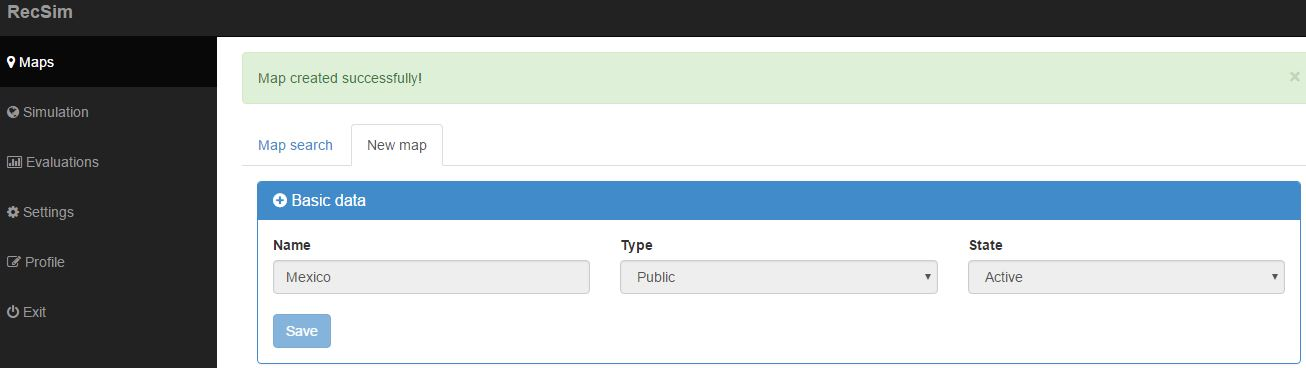
\includegraphics[scale=0.36]{imagenes/crear-mapa-nuevo-mexico.jpg}
	\caption{Creación de un mapa nuevo en México con datos reales}
	\label{mapaMexico}
\end{figure}

\subsection{Paso 3: crear un escenario realista}

La creación de escenarios funciona como un asistente de configuración. A continuación se muestra los pasos que hay que realizar para configurar un escenario realista:

\subsubsection{Paso 1: definir el nombre del escenario y elegir el recomendador}

En el primer paso de la creación de un escenario consiste en poner un nombre del escenario y elegir que recomendador vamos a usar en dicho escenario. En la figura \ref{paso1DefinirNombreYrecomendador} podemos una captura de este paso:

\begin{figure}[H]
	\centering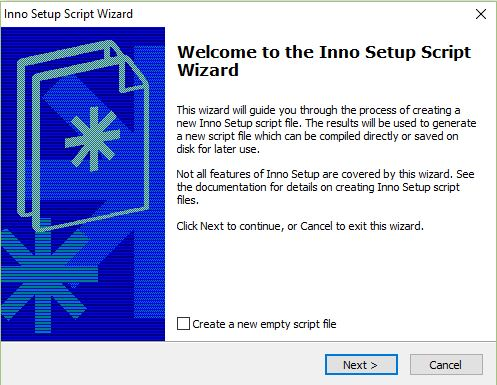
\includegraphics[scale=0.45]{imagenes/explotacion/1.jpg}
	\caption{Paso 1: definir un nombre y recomendador para el escenario realista}
	\label{paso1DefinirNombreYrecomendador}
\end{figure}

\subsubsection{Paso 2: definir los limites del escenario}

En segundo paso de la creación del escenario realista consiste en definir los limites geográficos del escenario. Por esto lo primero que tenemos que hacer es usar el buscador para buscar la ciudad donde se va a realizar la simulación. Una vez que hayamos encontrado y seleccionado la cuidad definiremos la esquina superior izquierda ya la esquina inferior derecha. En la figura \ref{paso2definirLimitesEscenarioRealista} vemos el resultado:

\begin{figure}[H]
	\centering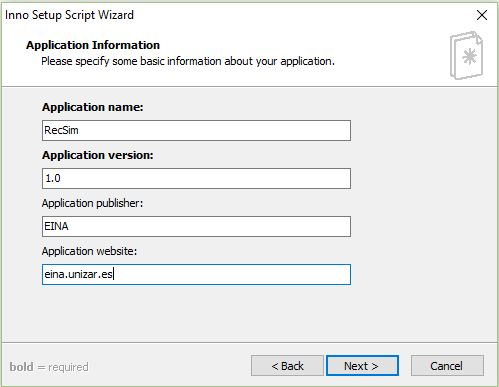
\includegraphics[scale=0.45]{imagenes/explotacion/2.jpg}
	\caption{Paso 2: definir los limites del escenario realista}
	\label{paso2definirLimitesEscenarioRealista}
\end{figure}

\subsubsection{Paso 3: importar los datos de los restaurantes}

El siguiente paso consiste definir los restaurantes. El simulador dispone de varias opciones mediante las cuales es posible hacer esto. Nosotros vamos a importar los restaurantes del fichero geoplaces2.csv que hemos descargado previamente. Antes de cargar los datos el contenido del fichero se pre visualiza en la pantalla (figura \ref{paso3definirLosRestaurantes})

\begin{figure}[H]
	\centering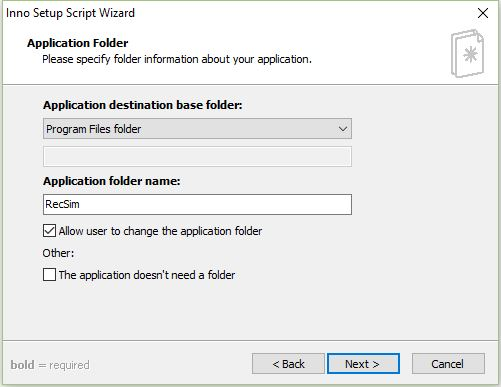
\includegraphics[scale=0.35]{imagenes/explotacion/3.jpg}
	\caption{Paso 3: definir los restaurantes sobre el escenario}
	\label{paso3definirLosRestaurantes}
\end{figure}

\newpage

Una vez importados los datos del fichero vemos que se muestra una lista con los restaurantes importados. Podemos ver esta lista con la figura \ref{paso31definirLosRestaurantes}:

\begin{figure}[H]
	\centering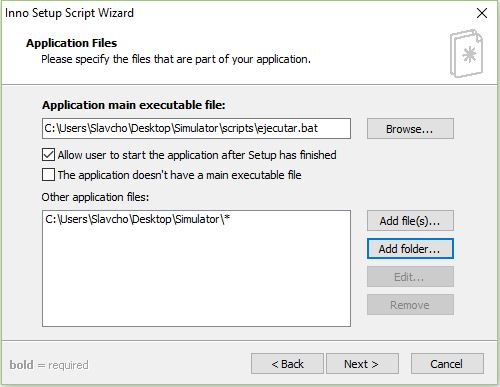
\includegraphics[scale=0.4]{imagenes/explotacion/4.jpg}
	\caption{Paso 3: lista de restaurantes definidos sobre el escenario}
	\label{paso31definirLosRestaurantes}
\end{figure}

\subsubsection{Paso 4: definir los objetos móviles}

El ultimo paso consiste en definir los objetos móviles. El simulador dispone de varias opciones mediante cuales se pueden definir objetos móviles. En este caso se han generado automáticamente (en la figura \ref{paso4ListaObjetosMoviles} podemos ver el resultado).

\begin{figure}[H]
	\centering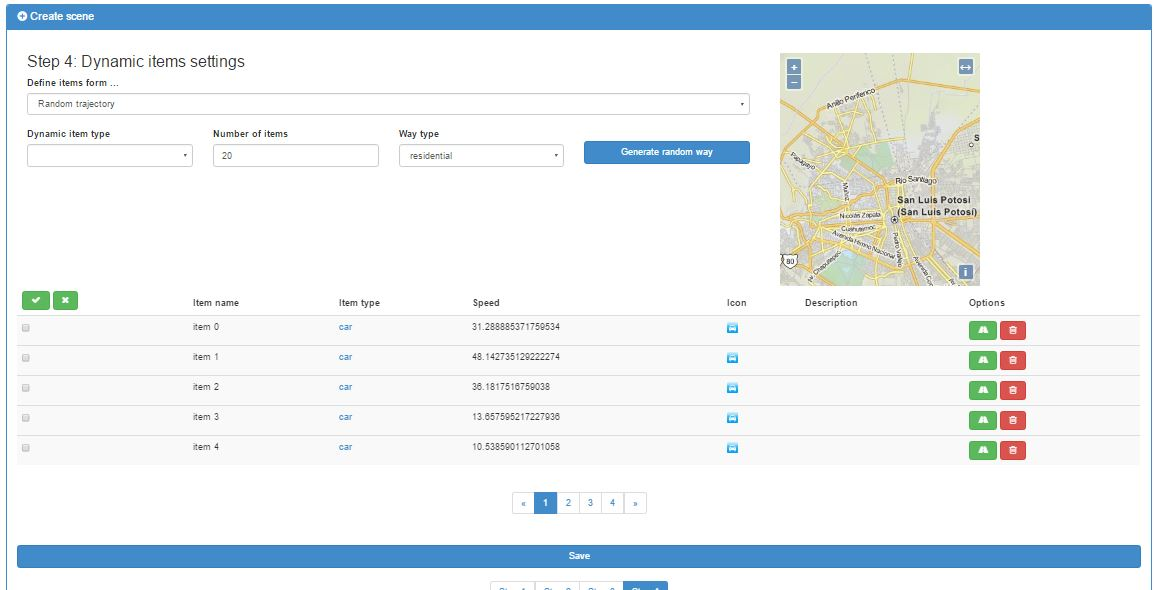
\includegraphics[scale=0.4]{imagenes/explotacion/5.jpg}
	\caption{Paso 4: lista de objetos móviles}
	\label{paso4ListaObjetosMoviles}
\end{figure}

\section{Simulación y evaluación de un sistema de recomendación}

\subsection{Simulación de un escenario realista}

Una vez que hayamos realizado la configuración del escenarios realista vamos a realizar simulaciones con dos usuarios y recoger las valoraciones que han realizado para su posterior evaluación. En la figura \ref{simulacionYEvaluacion} podemos ver una captura de una simulación realizada:

\begin{figure}[H]
	\centering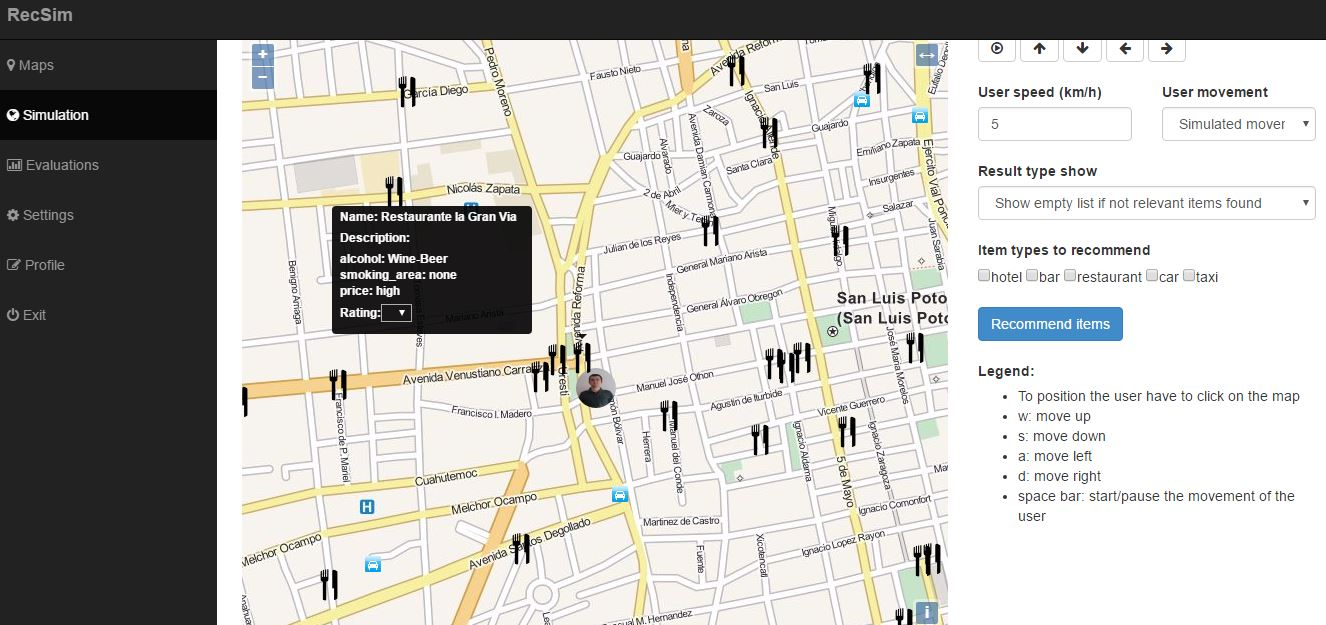
\includegraphics[scale=0.35]{imagenes/explotacion/6.jpg}
	\caption{Simulación realizada en San Luis Potosí, México}
	\label{simulacionYEvaluacion}
\end{figure}

\subsection{Evaluación de un recomendador}




\section{Rendimiento}

El limite teórico máximo de peticiones HTTP de las aplicaciones desarrolladas con Node.js es igual al número máximo de sockets que se puedan crear en el servidor, es decir, un servidor con un Sistema Operativo Linux puede crear 65535 sockets. Pero hay que tener en cuenta que una parte esta reservada para el Sistema Operativo. Esto nos deja entre 30.000 - 45.000 sockets que podemos usar. Tenemos que comprobar cómo se comporta el simulador y por lo tanto hemos realizado unas prueba de estrés tanto con Linux como con Windows.

\subsection{Rendimientos con Linux}

En este apartado se describe los resultados de las pruebas de estrés realizadas con un Sistema Operativo Linux con las siguientes características:

\begin{itemize}
	\item Sistema Operativo: Linux v15.10 64 bits
	\item RAM: 3.3 GB
	\item CPU: Intel i3 1.8 GHz
\end{itemize}

\begin{table}[H]
	\begin{center}
		\begin{tabular}{|c|c|c|c|c|c|}\hline
			Peticiones HTTP & CPU & Memoria & Kbytes/sec & Peticiones/seg & Segundos por petición \\ \hline
			50.000 & 24.8 & 134MB & 1593,86 & 508,76 & 0,196555 \\ \hline
			100.000 & 30.2 & 133 MB & 1716,46 & 547,89 & 0,182517 \\ \hline
			500.000 & 45.4 & 138MB & 1199,38 & 382,84 & 0,261204 \\ \hline
		\end{tabular}
		\caption{Pruebas de estrés con 100 usuarios concurrentes}
		\label{tabla:CienteUsuarios}
	\end{center}
\end{table}

\begin{table}[H]
	\begin{center}
		\begin{tabular}{|c|c|c|c|c|c|} 	\hline
			Peticiones HTTP & CPU & Memoria & Kbytes/sec & Peticiones/seg & Segundos por petición \\ \hline
			50.000 & 25.9 & 147MB & 1196,85 & 382,04 & 1,308774 \\ \hline
			100.000 & 40.6 & 160MB & 1286,86 & 410,78 & 1,2172 \\ \hline
			500.000 & 44.6 & 162 MB & n/d & n/d & n/d \\ \hline
		\end{tabular}
		\caption{Pruebas de estrés con 500 usuarios concurrentes}
		\label{tabla:QuinientosUsuarios}
	\end{center}
\end{table}

\begin{table}[H]
	\begin{center}
		\begin{tabular}{|c|c|c|c|c|c|} \hline
			Peticiones HTTP & CPU & Memoria & Kbytes/sec & Peticiones/seg & Segundos por petición \\ \hline
			50.000 & 24.3 & 160 MB & 1408,94 & 449,74 & 2,223517 \\ \hline
			100.000 & 26.3 & 167MB & n/d & n/d & n/d \\ \hline
			500.000 & n/d & n/d & n/d & n/d & n/d \\ \hline
		\end{tabular}
		\caption{Pruebas de estrés con 1000 usuarios concurrentes}
		\label{tabla:MilUsuarios}
	\end{center}
\end{table}

En el caso de la pruebas con 500 usuarios concurrentes nos da dado el error apr socket recv Connection timed out (110) y se han completado 105.195 peticiones HTTP en la prueba con 500.000 peticiones HTTP. En el caso de la prueba con 1000 usuarios concurrentes nos ha dado el mismo fallo que en el caso de los 500 usuarios concurrentes y se han completado 54.599 peticiones HTTP en la prueba con 100.000 peticiones HTTP. 

En el resto de casos las pruebas de carga han sido satisfactorias. Observamos que el peor de los casos se ha obtenido una media de 2,2 segundos por petición HTTP en el caso que tenemos 1000 usuarios concurrentes que han generado 50.000 peticiones HTTP.

\subsection{Rendimientos con Windows}

En este apartado se describe los resultados de las pruebas de estrés realizadas con un Sistema Operativo Windows con las siguientes características:

\begin{itemize}
	\item Sistema Operativo: Windows 10 Home 64 bits
	\item RAM: 8 GB
	\item CPU: Intel i3 1.8 GHz
\end{itemize}

\begin{lstlisting}[language=bash]
slavcho@ubuntu:~/testing$ ab -g resultados4.csv -n 50000 -c 100 http://192.168.1.102:81/
This is ApacheBench, Version 2.3 <$Revision: 1638069 $>
Copyright 1996 Adam Twiss, Zeus Technology Ltd, http://www.zeustech.net/
Licensed to The Apache Software Foundation, http://www.apache.org/

Benchmarking 192.168.1.102 (be patient)
Completed 5000 requests
Completed 10000 requests
Completed 15000 requests
apr_socket_recv: Connection timed out (110)
Total of 19219 requests completed
slavcho@ubuntu:~/testing$
\end{lstlisting}

\begin{lstlisting}[language=bash]
slavcho@ubuntu:~/testing$ ab -g resultados4.csv -n 50000 -c 500 http://192.168.1.102:81/
This is ApacheBench, Version 2.3 <$Revision: 1638069 $>
Copyright 1996 Adam Twiss, Zeus Technology Ltd, http://www.zeustech.net/
Licensed to The Apache Software Foundation, http://www.apache.org/

Benchmarking 192.168.1.102 (be patient)
apr_socket_recv: Connection refused (111)
Total of 558 requests completed
\end{lstlisting}


\begin{lstlisting}[language=bash]
slavcho@ubuntu:~/testing$ ab -g resultados4.csv -n 100000 -c 500 http://192.168.1.102:81/
This is ApacheBench, Version 2.3 <$Revision: 1638069 $>
Copyright 1996 Adam Twiss, Zeus Technology Ltd, http://www.zeustech.net/
Licensed to The Apache Software Foundation, http://www.apache.org/

Benchmarking 192.168.1.102 (be patient)
apr_socket_recv: Connection refused (111)
Total of 524 requests completed
\end{lstlisting}

En las pruebas realizadas observamos que nos ha dado fallo en todas las pruebas. En el caso de la prueba con 100 usuarios concurrentes 50.000 peticiones HTTP se ha completado 19.219 de las peticiones HTTP. En el caso de la prueba con 500 usuarios concurrentes y 50.000 peticiones HTTP se han completado 558 peticiones HTTP. En el caso de la prueba con 500 usuarios concurrentes y 100.000 peticiones HTTP se han completado 524 peticiones HTTP. 

\subsection{Conclusiones de las pruebas de estrés}

Como conclusión podemos determinar que el Sistema Operativo Linux se comporta bastante mejor que el Windows para esta aplicación. Por lo tanto recomiendo la utilización de un servidor Linux para el simulador de escenarios para aprovechar mejor tanto la aplicación como el hardware.